\documentclass[1p]{elsarticle_modified}
%\bibliographystyle{elsarticle-num}

%\usepackage[colorlinks]{hyperref}
%\usepackage{abbrmath_seonhwa} %\Abb, \Ascr, \Acal ,\Abf, \Afrak
\usepackage{amsfonts}
\usepackage{amssymb}
\usepackage{amsmath}
\usepackage{amsthm}
\usepackage{scalefnt}
\usepackage{amsbsy}
\usepackage{kotex}
\usepackage{caption}
\usepackage{subfig}
\usepackage{color}
\usepackage{graphicx}
\usepackage{xcolor} %% white, black, red, green, blue, cyan, magenta, yellow
\usepackage{float}
\usepackage{setspace}
\usepackage{hyperref}

\usepackage{tikz}
\usetikzlibrary{arrows}

\usepackage{multirow}
\usepackage{array} % fixed length table
\usepackage{hhline}

%%%%%%%%%%%%%%%%%%%%%
\makeatletter
\renewcommand*\env@matrix[1][\arraystretch]{%
	\edef\arraystretch{#1}%
	\hskip -\arraycolsep
	\let\@ifnextchar\new@ifnextchar
	\array{*\c@MaxMatrixCols c}}
\makeatother %https://tex.stackexchange.com/questions/14071/how-can-i-increase-the-line-spacing-in-a-matrix
%%%%%%%%%%%%%%%

\usepackage[normalem]{ulem}

\newcommand{\msout}[1]{\ifmmode\text{\sout{\ensuremath{#1}}}\else\sout{#1}\fi}
%SOURCE: \msout is \stkout macro in https://tex.stackexchange.com/questions/20609/strikeout-in-math-mode

\newcommand{\cancel}[1]{
	\ifmmode
	{\color{red}\msout{#1}}
	\else
	{\color{red}\sout{#1}}
	\fi
}

\newcommand{\add}[1]{
	{\color{blue}\uwave{#1}}
}

\newcommand{\replace}[2]{
	\ifmmode
	{\color{red}\msout{#1}}{\color{blue}\uwave{#2}}
	\else
	{\color{red}\sout{#1}}{\color{blue}\uwave{#2}}
	\fi
}

\newcommand{\Sol}{\mathcal{S}} %segment
\newcommand{\D}{D} %diagram
\newcommand{\A}{\mathcal{A}} %arc


%%%%%%%%%%%%%%%%%%%%%%%%%%%%%5 test

\def\sl{\operatorname{\textup{SL}}(2,\Cbb)}
\def\psl{\operatorname{\textup{PSL}}(2,\Cbb)}
\def\quan{\mkern 1mu \triangleright \mkern 1mu}

\theoremstyle{definition}
\newtheorem{thm}{Theorem}[section]
\newtheorem{prop}[thm]{Proposition}
\newtheorem{lem}[thm]{Lemma}
\newtheorem{ques}[thm]{Question}
\newtheorem{cor}[thm]{Corollary}
\newtheorem{defn}[thm]{Definition}
\newtheorem{exam}[thm]{Example}
\newtheorem{rmk}[thm]{Remark}
\newtheorem{alg}[thm]{Algorithm}

\newcommand{\I}{\sqrt{-1}}
\begin{document}

%\begin{frontmatter}
%
%\title{Boundary parabolic representations of knots up to 8 crossings}
%
%%% Group authors per affiliation:
%\author{Yunhi Cho} 
%\address{Department of Mathematics, University of Seoul, Seoul, Korea}
%\ead{yhcho@uos.ac.kr}
%
%
%\author{Seonhwa Kim} %\fnref{s_kim}}
%\address{Center for Geometry and Physics, Institute for Basic Science, Pohang, 37673, Korea}
%\ead{ryeona17@ibs.re.kr}
%
%\author{Hyuk Kim}
%\address{Department of Mathematical Sciences, Seoul National University, Seoul 08826, Korea}
%\ead{hyukkim@snu.ac.kr}
%
%\author{Seokbeom Yoon}
%\address{Department of Mathematical Sciences, Seoul National University, Seoul, 08826,  Korea}
%\ead{sbyoon15@snu.ac.kr}
%
%\begin{abstract}
%We find all boundary parabolic representation of knots up to 8 crossings.
%
%\end{abstract}
%\begin{keyword}
%    \MSC[2010] 57M25 
%\end{keyword}
%
%\end{frontmatter}

%\linenumbers
%\tableofcontents
%
\newcommand\colored[1]{\textcolor{white}{\rule[-0.35ex]{0.8em}{1.4ex}}\kern-0.8em\color{red} #1}%
%\newcommand\colored[1]{\textcolor{white}{ #1}\kern-2.17ex	\textcolor{white}{ #1}\kern-1.81ex	\textcolor{white}{ #1}\kern-2.15ex\color{red}#1	}

{\Large $\underline{12a_{0602}~(K12a_{0602})}$}

\setlength{\tabcolsep}{10pt}
\renewcommand{\arraystretch}{1.6}
\vspace{1cm}\begin{tabular}{m{100pt}>{\centering\arraybackslash}m{274pt}}
\multirow{5}{120pt}{
	\centering
	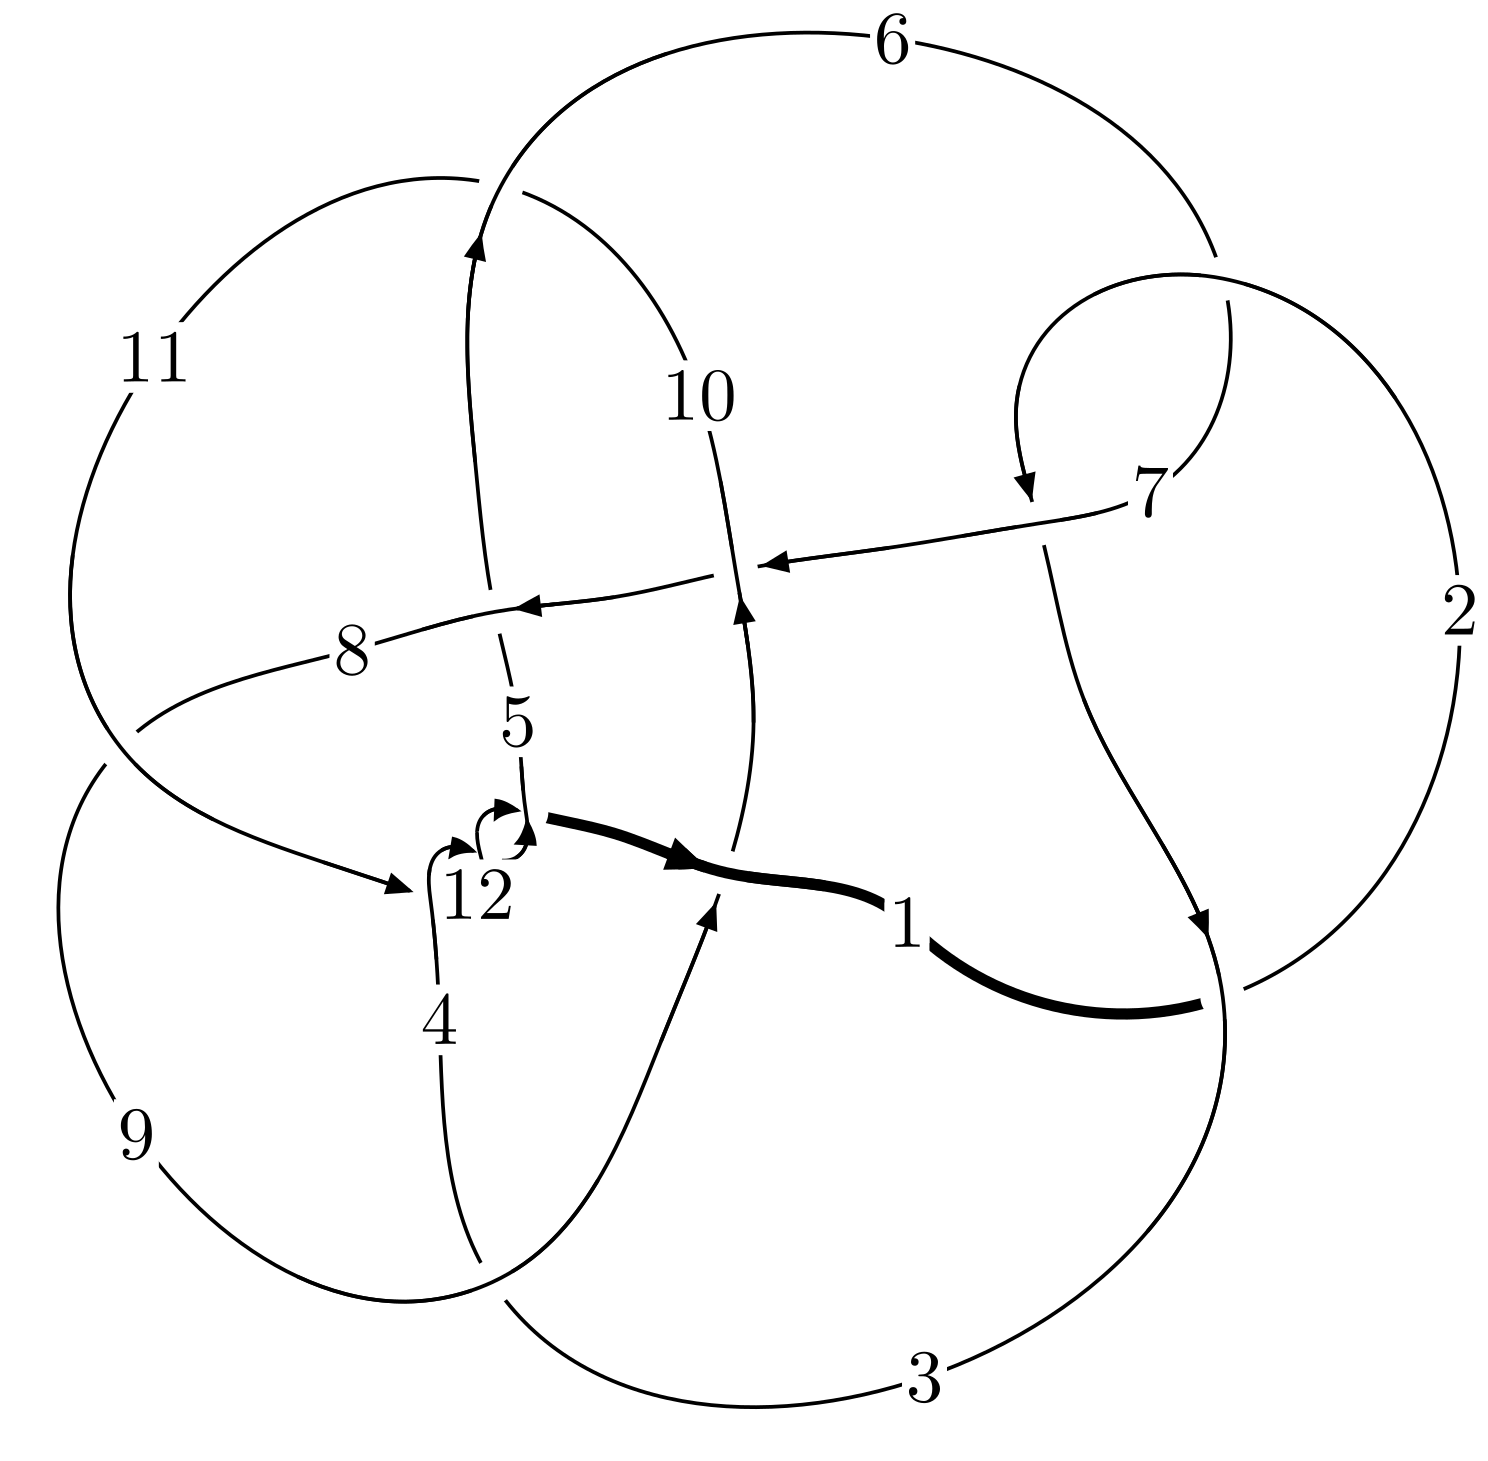
\includegraphics[width=112pt]{../../../GIT/diagram.site/Diagrams/png/1403_12a_0602.png}\\
\ \ \ A knot diagram\footnotemark}&
\allowdisplaybreaks
\textbf{Linearized knot diagam} \\
\cline{2-2}
 &
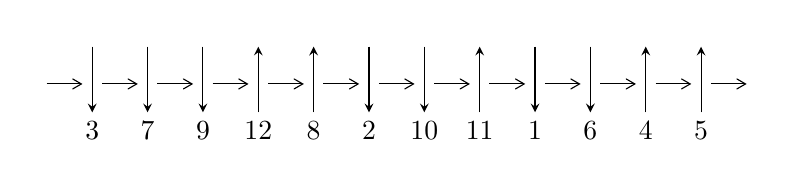
\begin{tikzpicture}[x=20pt, y=17pt]
	% nodes
	\node (C0) at (0, 0) {};
	\node (C1) at (1, 0) {};
	\node (C1U) at (1, +1) {};
	\node (C1D) at (1, -1) {3};

	\node (C2) at (2, 0) {};
	\node (C2U) at (2, +1) {};
	\node (C2D) at (2, -1) {7};

	\node (C3) at (3, 0) {};
	\node (C3U) at (3, +1) {};
	\node (C3D) at (3, -1) {9};

	\node (C4) at (4, 0) {};
	\node (C4U) at (4, +1) {};
	\node (C4D) at (4, -1) {12};

	\node (C5) at (5, 0) {};
	\node (C5U) at (5, +1) {};
	\node (C5D) at (5, -1) {8};

	\node (C6) at (6, 0) {};
	\node (C6U) at (6, +1) {};
	\node (C6D) at (6, -1) {2};

	\node (C7) at (7, 0) {};
	\node (C7U) at (7, +1) {};
	\node (C7D) at (7, -1) {10};

	\node (C8) at (8, 0) {};
	\node (C8U) at (8, +1) {};
	\node (C8D) at (8, -1) {11};

	\node (C9) at (9, 0) {};
	\node (C9U) at (9, +1) {};
	\node (C9D) at (9, -1) {1};

	\node (C10) at (10, 0) {};
	\node (C10U) at (10, +1) {};
	\node (C10D) at (10, -1) {6};

	\node (C11) at (11, 0) {};
	\node (C11U) at (11, +1) {};
	\node (C11D) at (11, -1) {4};

	\node (C12) at (12, 0) {};
	\node (C12U) at (12, +1) {};
	\node (C12D) at (12, -1) {5};
	\node (C13) at (13, 0) {};

	% arrows
	\draw[->,>={angle 60}]
	(C0) edge (C1) (C1) edge (C2) (C2) edge (C3) (C3) edge (C4) (C4) edge (C5) (C5) edge (C6) (C6) edge (C7) (C7) edge (C8) (C8) edge (C9) (C9) edge (C10) (C10) edge (C11) (C11) edge (C12) (C12) edge (C13) ;	\draw[->,>=stealth]
	(C1U) edge (C1D) (C2U) edge (C2D) (C3U) edge (C3D) (C4D) edge (C4U) (C5D) edge (C5U) (C6U) edge (C6D) (C7U) edge (C7D) (C8D) edge (C8U) (C9U) edge (C9D) (C10U) edge (C10D) (C11D) edge (C11U) (C12D) edge (C12U) ;
	\end{tikzpicture} \\
\hhline{~~} \\& 
\textbf{Solving Sequence} \\ \cline{2-2} 
 &
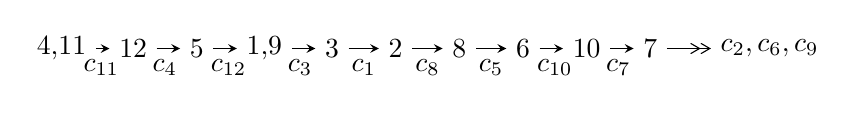
\begin{tikzpicture}[x=23pt, y=7pt]
	% node
	\node (A0) at (-1/8, 0) {4,11};
	\node (A1) at (1, 0) {12};
	\node (A2) at (2, 0) {5};
	\node (A3) at (49/16, 0) {1,9};
	\node (A4) at (33/8, 0) {3};
	\node (A5) at (41/8, 0) {2};
	\node (A6) at (49/8, 0) {8};
	\node (A7) at (57/8, 0) {6};
	\node (A8) at (65/8, 0) {10};
	\node (A9) at (73/8, 0) {7};
	\node (C1) at (1/2, -1) {$c_{11}$};
	\node (C2) at (3/2, -1) {$c_{4}$};
	\node (C3) at (5/2, -1) {$c_{12}$};
	\node (C4) at (29/8, -1) {$c_{3}$};
	\node (C5) at (37/8, -1) {$c_{1}$};
	\node (C6) at (45/8, -1) {$c_{8}$};
	\node (C7) at (53/8, -1) {$c_{5}$};
	\node (C8) at (61/8, -1) {$c_{10}$};
	\node (C9) at (69/8, -1) {$c_{7}$};
	\node (A10) at (11, 0) {$c_{2},c_{6},c_{9}$};

	% edge
	\draw[->,>=stealth]	
	(A0) edge (A1) (A1) edge (A2) (A2) edge (A3) (A3) edge (A4) (A4) edge (A5) (A5) edge (A6) (A6) edge (A7) (A7) edge (A8) (A8) edge (A9) ;
	\draw[->>,>={angle 60}]	
	(A9) edge (A10);
\end{tikzpicture} \\ 

\end{tabular} \\

\footnotetext{
The image of knot diagram is generated by the software ``\textbf{Draw programme}" developed by Andrew Bartholomew(\url{http://www.layer8.co.uk/maths/draw/index.htm\#Running-draw}), where we modified some parts for our purpose(\url{https://github.com/CATsTAILs/LinksPainter}).
}\phantom \\ \newline 
\centering \textbf{Ideals for irreducible components\footnotemark of $X_{\text{par}}$} 
 
\begin{align*}
I^u_{1}&=\langle 
4.66581\times10^{374} u^{143}-1.28668\times10^{375} u^{142}+\cdots+1.64873\times10^{373} b-4.11352\times10^{374},\\
\phantom{I^u_{1}}&\phantom{= \langle  }-7.48886\times10^{372} u^{143}+1.93957\times10^{373} u^{142}+\cdots+1.49885\times10^{372} a+3.95483\times10^{372},\\
\phantom{I^u_{1}}&\phantom{= \langle  }u^{144}-4 u^{143}+\cdots+15 u+1\rangle \\
I^u_{2}&=\langle 
-20959 u^{29}-11090 u^{28}+\cdots+149 b+20698,\;-3 u^{29}+u^{28}+\cdots+a+11,\;u^{30}- u^{29}+\cdots-4 u+1\rangle \\
\\
\end{align*}
\raggedright * 2 irreducible components of $\dim_{\mathbb{C}}=0$, with total 174 representations.\\
\footnotetext{All coefficients of polynomials are rational numbers. But the coefficients are sometimes approximated in decimal forms when there is not enough margin.}
\newpage
\renewcommand{\arraystretch}{1}
\centering \section*{I. $I^u_{1}= \langle 4.67\times10^{374} u^{143}-1.29\times10^{375} u^{142}+\cdots+1.65\times10^{373} b-4.11\times10^{374},\;-7.49\times10^{372} u^{143}+1.94\times10^{373} u^{142}+\cdots+1.50\times10^{372} a+3.95\times10^{372},\;u^{144}-4 u^{143}+\cdots+15 u+1 \rangle$}
\flushleft \textbf{(i) Arc colorings}\\
\begin{tabular}{m{7pt} m{180pt} m{7pt} m{180pt} }
\flushright $a_{4}=$&$\begin{pmatrix}0\\u\end{pmatrix}$ \\
\flushright $a_{11}=$&$\begin{pmatrix}1\\0\end{pmatrix}$ \\
\flushright $a_{12}=$&$\begin{pmatrix}1\\- u^2\end{pmatrix}$ \\
\flushright $a_{5}=$&$\begin{pmatrix}u\\- u^3+u\end{pmatrix}$ \\
\flushright $a_{1}=$&$\begin{pmatrix}- u^2+1\\u^4-2 u^2\end{pmatrix}$ \\
\flushright $a_{9}=$&$\begin{pmatrix}4.99642 u^{143}-12.9404 u^{142}+\cdots-214.068 u-2.63858\\-28.2994 u^{143}+78.0404 u^{142}+\cdots+375.005 u+24.9496\end{pmatrix}$ \\
\flushright $a_{3}=$&$\begin{pmatrix}19.6393 u^{143}-58.9874 u^{142}+\cdots+30.6121 u+2.17158\\-34.0052 u^{143}+94.0370 u^{142}+\cdots+484.569 u+29.7387\end{pmatrix}$ \\
\flushright $a_{2}=$&$\begin{pmatrix}18.4548 u^{143}-50.7937 u^{142}+\cdots-206.122 u-23.9926\\20.1291 u^{143}-56.0029 u^{142}+\cdots-273.396 u-18.6684\end{pmatrix}$ \\
\flushright $a_{8}=$&$\begin{pmatrix}33.2958 u^{143}-90.9809 u^{142}+\cdots-589.073 u-27.5882\\-28.2994 u^{143}+78.0404 u^{142}+\cdots+375.005 u+24.9496\end{pmatrix}$ \\
\flushright $a_{6}=$&$\begin{pmatrix}20.9047 u^{143}-60.8386 u^{142}+\cdots-85.9031 u-3.42492\\-7.44544 u^{143}+21.2506 u^{142}+\cdots+128.326 u+7.67264\end{pmatrix}$ \\
\flushright $a_{10}=$&$\begin{pmatrix}14.8061 u^{143}-39.8561 u^{142}+\cdots-366.170 u-13.3050\\-12.0229 u^{143}+32.9768 u^{142}+\cdots+161.382 u+11.4844\end{pmatrix}$ \\
\flushright $a_{7}=$&$\begin{pmatrix}-16.2278 u^{143}+46.8176 u^{142}+\cdots+183.885 u+25.5784\\-15.2646 u^{143}+42.8316 u^{142}+\cdots+229.429 u+16.3077\end{pmatrix}$\\&\end{tabular}
\flushleft \textbf{(ii) Obstruction class $= -1$}\\~\\
\flushleft \textbf{(iii) Cusp Shapes $= -34.9261 u^{143}+102.204 u^{142}+\cdots+484.487 u+41.1578$}\\~\\
\newpage\renewcommand{\arraystretch}{1}
\flushleft \textbf{(iv) u-Polynomials at the component}\newline \\
\begin{tabular}{m{50pt}|m{274pt}}
Crossings & \hspace{64pt}u-Polynomials at each crossing \\
\hline $$\begin{aligned}c_{1}\end{aligned}$$&$\begin{aligned}
&u^{144}+58 u^{143}+\cdots+11398 u+361
\end{aligned}$\\
\hline $$\begin{aligned}c_{2},c_{6}\end{aligned}$$&$\begin{aligned}
&u^{144}-2 u^{143}+\cdots+32 u+19
\end{aligned}$\\
\hline $$\begin{aligned}c_{3}\end{aligned}$$&$\begin{aligned}
&u^{144}-2 u^{143}+\cdots-340955512 u+126824923
\end{aligned}$\\
\hline $$\begin{aligned}c_{4},c_{11},c_{12}\end{aligned}$$&$\begin{aligned}
&u^{144}-4 u^{143}+\cdots+15 u+1
\end{aligned}$\\
\hline $$\begin{aligned}c_{5}\end{aligned}$$&$\begin{aligned}
&u^{144}+15 u^{143}+\cdots+45 u-1
\end{aligned}$\\
\hline $$\begin{aligned}c_{7}\end{aligned}$$&$\begin{aligned}
&u^{144}+2 u^{143}+\cdots-74 u+7
\end{aligned}$\\
\hline $$\begin{aligned}c_{8}\end{aligned}$$&$\begin{aligned}
&u^{144}-14 u^{143}+\cdots-235130 u+65317
\end{aligned}$\\
\hline $$\begin{aligned}c_{9}\end{aligned}$$&$\begin{aligned}
&u^{144}- u^{143}+\cdots-2778440 u+233557
\end{aligned}$\\
\hline $$\begin{aligned}c_{10}\end{aligned}$$&$\begin{aligned}
&u^{144}+5 u^{143}+\cdots-140899 u+14783
\end{aligned}$\\
\hline
\end{tabular}\\~\\
\newpage\renewcommand{\arraystretch}{1}
\flushleft \textbf{(v) Riley Polynomials at the component}\newline \\
\begin{tabular}{m{50pt}|m{274pt}}
Crossings & \hspace{64pt}Riley Polynomials at each crossing \\
\hline $$\begin{aligned}c_{1}\end{aligned}$$&$\begin{aligned}
&y^{144}+70 y^{143}+\cdots+11864014 y+130321
\end{aligned}$\\
\hline $$\begin{aligned}c_{2},c_{6}\end{aligned}$$&$\begin{aligned}
&y^{144}-58 y^{143}+\cdots-11398 y+361
\end{aligned}$\\
\hline $$\begin{aligned}c_{3}\end{aligned}$$&$\begin{aligned}
&y^{144}+50 y^{143}+\cdots+928165311949487672 y+16084561093955929
\end{aligned}$\\
\hline $$\begin{aligned}c_{4},c_{11},c_{12}\end{aligned}$$&$\begin{aligned}
&y^{144}-142 y^{143}+\cdots+159 y+1
\end{aligned}$\\
\hline $$\begin{aligned}c_{5}\end{aligned}$$&$\begin{aligned}
&y^{144}+5 y^{143}+\cdots-3139 y+1
\end{aligned}$\\
\hline $$\begin{aligned}c_{7}\end{aligned}$$&$\begin{aligned}
&y^{144}+12 y^{143}+\cdots+1734 y+49
\end{aligned}$\\
\hline $$\begin{aligned}c_{8}\end{aligned}$$&$\begin{aligned}
&y^{144}-44 y^{143}+\cdots+923597554320 y+4266310489
\end{aligned}$\\
\hline $$\begin{aligned}c_{9}\end{aligned}$$&$\begin{aligned}
&y^{144}+29 y^{143}+\cdots+159556190882 y+54548872249
\end{aligned}$\\
\hline $$\begin{aligned}c_{10}\end{aligned}$$&$\begin{aligned}
&y^{144}+25 y^{143}+\cdots+5445649265 y+218537089
\end{aligned}$\\
\hline
\end{tabular}\\~\\
\newpage\flushleft \textbf{(vi) Complex Volumes and Cusp Shapes}
$$\begin{array}{c|c|c}  
\text{Solutions to }I^u_{1}& \I (\text{vol} + \sqrt{-1}CS) & \text{Cusp shape}\\
 \hline 
\begin{aligned}
u &= -0.641440 + 0.771294 I \\
a &= \phantom{-}0.243379 - 0.887983 I \\
b &= \phantom{-}0.406077 - 0.706504 I\end{aligned}
 & -1.32437 - 6.15069 I & \phantom{-0.000000 } 0 \\ \hline\begin{aligned}
u &= -0.641440 - 0.771294 I \\
a &= \phantom{-}0.243379 + 0.887983 I \\
b &= \phantom{-}0.406077 + 0.706504 I\end{aligned}
 & -1.32437 + 6.15069 I & \phantom{-0.000000 } 0 \\ \hline\begin{aligned}
u &= \phantom{-}0.436258 + 0.919189 I \\
a &= -0.572363 - 0.544707 I \\
b &= -1.079820 - 0.266336 I\end{aligned}
 & \phantom{-}2.33630 + 3.72932 I & \phantom{-0.000000 } 0 \\ \hline\begin{aligned}
u &= \phantom{-}0.436258 - 0.919189 I \\
a &= -0.572363 + 0.544707 I \\
b &= -1.079820 + 0.266336 I\end{aligned}
 & \phantom{-}2.33630 - 3.72932 I & \phantom{-0.000000 } 0 \\ \hline\begin{aligned}
u &= \phantom{-}0.708847 + 0.732712 I \\
a &= -0.955680 - 0.457394 I \\
b &= -0.973986 + 0.386429 I\end{aligned}
 & \phantom{-}4.03243 - 3.94384 I & \phantom{-0.000000 } 0 \\ \hline\begin{aligned}
u &= \phantom{-}0.708847 - 0.732712 I \\
a &= -0.955680 + 0.457394 I \\
b &= -0.973986 - 0.386429 I\end{aligned}
 & \phantom{-}4.03243 + 3.94384 I & \phantom{-0.000000 } 0 \\ \hline\begin{aligned}
u &= -0.704071 + 0.749730 I \\
a &= -1.075930 + 0.332157 I \\
b &= -0.991888 - 0.473815 I\end{aligned}
 & \phantom{-}2.28410 + 9.91942 I & \phantom{-0.000000 } 0 \\ \hline\begin{aligned}
u &= -0.704071 - 0.749730 I \\
a &= -1.075930 - 0.332157 I \\
b &= -0.991888 + 0.473815 I\end{aligned}
 & \phantom{-}2.28410 - 9.91942 I & \phantom{-0.000000 } 0 \\ \hline\begin{aligned}
u &= \phantom{-}0.940999 + 0.434490 I \\
a &= \phantom{-}0.359772 + 0.263997 I \\
b &= -0.053654 - 0.152778 I\end{aligned}
 & \phantom{-}1.59960 + 1.70116 I & \phantom{-0.000000 } 0 \\ \hline\begin{aligned}
u &= \phantom{-}0.940999 - 0.434490 I \\
a &= \phantom{-}0.359772 - 0.263997 I \\
b &= -0.053654 + 0.152778 I\end{aligned}
 & \phantom{-}1.59960 - 1.70116 I & \phantom{-0.000000 } 0\\
 \hline 
 \end{array}$$\newpage$$\begin{array}{c|c|c}  
\text{Solutions to }I^u_{1}& \I (\text{vol} + \sqrt{-1}CS) & \text{Cusp shape}\\
 \hline 
\begin{aligned}
u &= -0.464501 + 0.837838 I \\
a &= -0.407758 + 1.133410 I \\
b &= -0.976569 + 0.678738 I\end{aligned}
 & -3.88117 - 7.32238 I & \phantom{-0.000000 } 0 \\ \hline\begin{aligned}
u &= -0.464501 - 0.837838 I \\
a &= -0.407758 - 1.133410 I \\
b &= -0.976569 - 0.678738 I\end{aligned}
 & -3.88117 + 7.32238 I & \phantom{-0.000000 } 0 \\ \hline\begin{aligned}
u &= -0.463367 + 0.837097 I \\
a &= -0.77191 + 1.38289 I \\
b &= -1.24742 + 0.82437 I\end{aligned}
 & \phantom{-}1.5784 - 15.2624 I & \phantom{-0.000000 } 0 \\ \hline\begin{aligned}
u &= -0.463367 - 0.837097 I \\
a &= -0.77191 - 1.38289 I \\
b &= -1.24742 - 0.82437 I\end{aligned}
 & \phantom{-}1.5784 + 15.2624 I & \phantom{-0.000000 } 0 \\ \hline\begin{aligned}
u &= \phantom{-}0.459927 + 0.835725 I \\
a &= -0.78045 - 1.24759 I \\
b &= -1.24228 - 0.73144 I\end{aligned}
 & \phantom{-}3.29096 + 9.25039 I & \phantom{-0.000000 } 0 \\ \hline\begin{aligned}
u &= \phantom{-}0.459927 - 0.835725 I \\
a &= -0.78045 + 1.24759 I \\
b &= -1.24228 + 0.73144 I\end{aligned}
 & \phantom{-}3.29096 - 9.25039 I & \phantom{-0.000000 } 0 \\ \hline\begin{aligned}
u &= -0.371568 + 0.988700 I \\
a &= \phantom{-}0.544420 - 0.388172 I \\
b &= \phantom{-}0.451860 - 0.236766 I\end{aligned}
 & -2.71360 + 0.49612 I & \phantom{-0.000000 } 0 \\ \hline\begin{aligned}
u &= -0.371568 - 0.988700 I \\
a &= \phantom{-}0.544420 + 0.388172 I \\
b &= \phantom{-}0.451860 + 0.236766 I\end{aligned}
 & -2.71360 - 0.49612 I & \phantom{-0.000000 } 0 \\ \hline\begin{aligned}
u &= -0.752384 + 0.751617 I \\
a &= -0.525272 + 0.180553 I \\
b &= -0.699403 - 0.333217 I\end{aligned}
 & -3.10082 + 1.92208 I & \phantom{-0.000000 } 0 \\ \hline\begin{aligned}
u &= -0.752384 - 0.751617 I \\
a &= -0.525272 - 0.180553 I \\
b &= -0.699403 + 0.333217 I\end{aligned}
 & -3.10082 - 1.92208 I & \phantom{-0.000000 } 0\\
 \hline 
 \end{array}$$\newpage$$\begin{array}{c|c|c}  
\text{Solutions to }I^u_{1}& \I (\text{vol} + \sqrt{-1}CS) & \text{Cusp shape}\\
 \hline 
\begin{aligned}
u &= \phantom{-}0.724474 + 0.503590 I \\
a &= -0.123746 - 1.223240 I \\
b &= -0.864459 + 0.063741 I\end{aligned}
 & \phantom{-}3.89536 + 1.41739 I & \phantom{-0.000000 } 0 \\ \hline\begin{aligned}
u &= \phantom{-}0.724474 - 0.503590 I \\
a &= -0.123746 + 1.223240 I \\
b &= -0.864459 - 0.063741 I\end{aligned}
 & \phantom{-}3.89536 - 1.41739 I & \phantom{-0.000000 } 0 \\ \hline\begin{aligned}
u &= \phantom{-}0.616552 + 0.598068 I \\
a &= \phantom{-}0.435778 + 1.109760 I \\
b &= \phantom{-}0.730539 + 0.818723 I\end{aligned}
 & \phantom{-}0.10188 + 2.22655 I & \phantom{-0.000000 } 0 \\ \hline\begin{aligned}
u &= \phantom{-}0.616552 - 0.598068 I \\
a &= \phantom{-}0.435778 - 1.109760 I \\
b &= \phantom{-}0.730539 - 0.818723 I\end{aligned}
 & \phantom{-}0.10188 - 2.22655 I & \phantom{-0.000000 } 0 \\ \hline\begin{aligned}
u &= -1.148590 + 0.085619 I \\
a &= \phantom{-}0.862771 - 0.704486 I \\
b &= \phantom{-}0.401690 - 0.881219 I\end{aligned}
 & \phantom{-}2.40569 - 1.29967 I & \phantom{-0.000000 } 0 \\ \hline\begin{aligned}
u &= -1.148590 - 0.085619 I \\
a &= \phantom{-}0.862771 + 0.704486 I \\
b &= \phantom{-}0.401690 + 0.881219 I\end{aligned}
 & \phantom{-}2.40569 + 1.29967 I & \phantom{-0.000000 } 0 \\ \hline\begin{aligned}
u &= \phantom{-}0.753275 + 0.380915 I \\
a &= \phantom{-}0.686476 + 0.925921 I \\
b &= \phantom{-}0.903434 + 0.867411 I\end{aligned}
 & \phantom{-}1.80300 + 6.03304 I & \phantom{-0.000000 } 0 \\ \hline\begin{aligned}
u &= \phantom{-}0.753275 - 0.380915 I \\
a &= \phantom{-}0.686476 - 0.925921 I \\
b &= \phantom{-}0.903434 - 0.867411 I\end{aligned}
 & \phantom{-}1.80300 - 6.03304 I & \phantom{-0.000000 } 0 \\ \hline\begin{aligned}
u &= \phantom{-}0.460385 + 0.689496 I \\
a &= \phantom{-}0.678854 + 0.951544 I \\
b &= \phantom{-}0.745760 + 0.518700 I\end{aligned}
 & \phantom{-}0.46793 + 2.15742 I & \phantom{-0.000000 } 0 \\ \hline\begin{aligned}
u &= \phantom{-}0.460385 - 0.689496 I \\
a &= \phantom{-}0.678854 - 0.951544 I \\
b &= \phantom{-}0.745760 - 0.518700 I\end{aligned}
 & \phantom{-}0.46793 - 2.15742 I & \phantom{-0.000000 } 0\\
 \hline 
 \end{array}$$\newpage$$\begin{array}{c|c|c}  
\text{Solutions to }I^u_{1}& \I (\text{vol} + \sqrt{-1}CS) & \text{Cusp shape}\\
 \hline 
\begin{aligned}
u &= \phantom{-}1.177910 + 0.025403 I \\
a &= \phantom{-}0.790502 - 1.020010 I \\
b &= \phantom{-}0.365064 - 1.132200 I\end{aligned}
 & \phantom{-}1.72067 - 5.51367 I & \phantom{-0.000000 } 0 \\ \hline\begin{aligned}
u &= \phantom{-}1.177910 - 0.025403 I \\
a &= \phantom{-}0.790502 + 1.020010 I \\
b &= \phantom{-}0.365064 + 1.132200 I\end{aligned}
 & \phantom{-}1.72067 + 5.51367 I & \phantom{-0.000000 } 0 \\ \hline\begin{aligned}
u &= -0.183903 + 0.780009 I \\
a &= -0.824077 - 0.031941 I \\
b &= -1.206750 - 0.054712 I\end{aligned}
 & \phantom{-}0.70996 + 3.48348 I & \phantom{-0.000000 } 0 \\ \hline\begin{aligned}
u &= -0.183903 - 0.780009 I \\
a &= -0.824077 + 0.031941 I \\
b &= -1.206750 + 0.054712 I\end{aligned}
 & \phantom{-}0.70996 - 3.48348 I & \phantom{-0.000000 } 0 \\ \hline\begin{aligned}
u &= \phantom{-}1.211750 + 0.000729 I \\
a &= \phantom{-}0.771860 + 0.326502 I \\
b &= -0.841770 - 0.766189 I\end{aligned}
 & \phantom{-}3.67045 - 0.65197 I & \phantom{-0.000000 } 0 \\ \hline\begin{aligned}
u &= \phantom{-}1.211750 - 0.000729 I \\
a &= \phantom{-}0.771860 - 0.326502 I \\
b &= -0.841770 + 0.766189 I\end{aligned}
 & \phantom{-}3.67045 + 0.65197 I & \phantom{-0.000000 } 0 \\ \hline\begin{aligned}
u &= -0.420892 + 0.635724 I \\
a &= \phantom{-}0.622376 + 0.623430 I \\
b &= -0.210982 + 0.432938 I\end{aligned}
 & -2.01335 + 1.40917 I & \phantom{-0.000000 } 0 \\ \hline\begin{aligned}
u &= -0.420892 - 0.635724 I \\
a &= \phantom{-}0.622376 - 0.623430 I \\
b &= -0.210982 - 0.432938 I\end{aligned}
 & -2.01335 - 1.40917 I & \phantom{-0.000000 } 0 \\ \hline\begin{aligned}
u &= -1.033270 + 0.685139 I \\
a &= \phantom{-}0.129460 - 0.303563 I \\
b &= \phantom{-}0.0254407 - 0.1005390 I\end{aligned}
 & -0.88369 - 6.44136 I & \phantom{-0.000000 } 0 \\ \hline\begin{aligned}
u &= -1.033270 - 0.685139 I \\
a &= \phantom{-}0.129460 + 0.303563 I \\
b &= \phantom{-}0.0254407 + 0.1005390 I\end{aligned}
 & -0.88369 + 6.44136 I & \phantom{-0.000000 } 0\\
 \hline 
 \end{array}$$\newpage$$\begin{array}{c|c|c}  
\text{Solutions to }I^u_{1}& \I (\text{vol} + \sqrt{-1}CS) & \text{Cusp shape}\\
 \hline 
\begin{aligned}
u &= -0.594458 + 0.471215 I \\
a &= -0.10005 + 1.82899 I \\
b &= -0.850397 + 0.092402 I\end{aligned}
 & \phantom{-}2.24619 - 7.45474 I & \phantom{-0.000000 } 0 \\ \hline\begin{aligned}
u &= -0.594458 - 0.471215 I \\
a &= -0.10005 - 1.82899 I \\
b &= -0.850397 - 0.092402 I\end{aligned}
 & \phantom{-}2.24619 + 7.45474 I & \phantom{-0.000000 } 0 \\ \hline\begin{aligned}
u &= -0.712997 + 0.244476 I \\
a &= \phantom{-}0.695977 - 0.637100 I \\
b &= \phantom{-}0.908432 - 0.844981 I\end{aligned}
 & \phantom{-}2.18454 - 1.39541 I & \phantom{-0.000000 } 0 \\ \hline\begin{aligned}
u &= -0.712997 - 0.244476 I \\
a &= \phantom{-}0.695977 + 0.637100 I \\
b &= \phantom{-}0.908432 + 0.844981 I\end{aligned}
 & \phantom{-}2.18454 + 1.39541 I & \phantom{-0.000000 } 0 \\ \hline\begin{aligned}
u &= \phantom{-}0.026738 + 0.749032 I \\
a &= \phantom{-}1.73714 - 0.12287 I \\
b &= \phantom{-}0.537774 - 0.089173 I\end{aligned}
 & -0.77627 - 2.15652 I & \phantom{-0.000000 } 0 \\ \hline\begin{aligned}
u &= \phantom{-}0.026738 - 0.749032 I \\
a &= \phantom{-}1.73714 + 0.12287 I \\
b &= \phantom{-}0.537774 + 0.089173 I\end{aligned}
 & -0.77627 + 2.15652 I & \phantom{-0.000000 } 0 \\ \hline\begin{aligned}
u &= -1.251690 + 0.018135 I \\
a &= \phantom{-}0.947540 - 0.308619 I \\
b &= -1.28552 + 0.93185 I\end{aligned}
 & \phantom{-}2.56527 + 6.04434 I & \phantom{-0.000000 } 0 \\ \hline\begin{aligned}
u &= -1.251690 - 0.018135 I \\
a &= \phantom{-}0.947540 + 0.308619 I \\
b &= -1.28552 - 0.93185 I\end{aligned}
 & \phantom{-}2.56527 - 6.04434 I & \phantom{-0.000000 } 0 \\ \hline\begin{aligned}
u &= -1.27165\phantom{ +0.000000I} \\
a &= \phantom{-}0.974017\phantom{ +0.000000I} \\
b &= -1.53369\phantom{ +0.000000I}\end{aligned}
 & -1.61073\phantom{ +0.000000I} & \phantom{-0.000000 } 0 \\ \hline\begin{aligned}
u &= -1.277810 + 0.176299 I \\
a &= \phantom{-}0.860025 - 0.120417 I \\
b &= -0.060909 - 0.274790 I\end{aligned}
 & \phantom{-}2.95543 - 4.81131 I & \phantom{-0.000000 } 0\\
 \hline 
 \end{array}$$\newpage$$\begin{array}{c|c|c}  
\text{Solutions to }I^u_{1}& \I (\text{vol} + \sqrt{-1}CS) & \text{Cusp shape}\\
 \hline 
\begin{aligned}
u &= -1.277810 - 0.176299 I \\
a &= \phantom{-}0.860025 + 0.120417 I \\
b &= -0.060909 + 0.274790 I\end{aligned}
 & \phantom{-}2.95543 + 4.81131 I & \phantom{-0.000000 } 0 \\ \hline\begin{aligned}
u &= \phantom{-}0.383418 + 0.595687 I \\
a &= \phantom{-}1.01919 + 1.97315 I \\
b &= \phantom{-}1.26345 + 0.79706 I\end{aligned}
 & \phantom{-}2.99110 + 1.22715 I & \phantom{-0.000000 } 0 \\ \hline\begin{aligned}
u &= \phantom{-}0.383418 - 0.595687 I \\
a &= \phantom{-}1.01919 - 1.97315 I \\
b &= \phantom{-}1.26345 - 0.79706 I\end{aligned}
 & \phantom{-}2.99110 - 1.22715 I & \phantom{-0.000000 } 0 \\ \hline\begin{aligned}
u &= -0.358887 + 0.592436 I \\
a &= \phantom{-}0.79562 - 2.24481 I \\
b &= \phantom{-}1.21593 - 0.95696 I\end{aligned}
 & \phantom{-}2.65144 - 6.14201 I & \phantom{-0.000000 } 0 \\ \hline\begin{aligned}
u &= -0.358887 - 0.592436 I \\
a &= \phantom{-}0.79562 + 2.24481 I \\
b &= \phantom{-}1.21593 + 0.95696 I\end{aligned}
 & \phantom{-}2.65144 + 6.14201 I & \phantom{-0.000000 } 0 \\ \hline\begin{aligned}
u &= \phantom{-}1.317590 + 0.046842 I \\
a &= \phantom{-}0.239324 - 1.329470 I \\
b &= \phantom{-}0.274809 - 1.056690 I\end{aligned}
 & \phantom{-}0.356643 + 0.438281 I & \phantom{-0.000000 } 0 \\ \hline\begin{aligned}
u &= \phantom{-}1.317590 - 0.046842 I \\
a &= \phantom{-}0.239324 + 1.329470 I \\
b &= \phantom{-}0.274809 + 1.056690 I\end{aligned}
 & \phantom{-}0.356643 - 0.438281 I & \phantom{-0.000000 } 0 \\ \hline\begin{aligned}
u &= \phantom{-}1.316210 + 0.092721 I \\
a &= \phantom{-}0.703686 - 0.065750 I \\
b &= -0.577824 + 0.200718 I\end{aligned}
 & \phantom{-}3.44128 + 0.54013 I & \phantom{-0.000000 } 0 \\ \hline\begin{aligned}
u &= \phantom{-}1.316210 - 0.092721 I \\
a &= \phantom{-}0.703686 + 0.065750 I \\
b &= -0.577824 - 0.200718 I\end{aligned}
 & \phantom{-}3.44128 - 0.54013 I & \phantom{-0.000000 } 0 \\ \hline\begin{aligned}
u &= \phantom{-}0.158197 + 0.659478 I \\
a &= \phantom{-}1.284820 - 0.499093 I \\
b &= \phantom{-}0.214700 - 0.361745 I\end{aligned}
 & -1.36302 + 1.81030 I & \phantom{-0.000000 } 0\\
 \hline 
 \end{array}$$\newpage$$\begin{array}{c|c|c}  
\text{Solutions to }I^u_{1}& \I (\text{vol} + \sqrt{-1}CS) & \text{Cusp shape}\\
 \hline 
\begin{aligned}
u &= \phantom{-}0.158197 - 0.659478 I \\
a &= \phantom{-}1.284820 + 0.499093 I \\
b &= \phantom{-}0.214700 + 0.361745 I\end{aligned}
 & -1.36302 - 1.81030 I & \phantom{-0.000000 } 0 \\ \hline\begin{aligned}
u &= -1.324880 + 0.039870 I \\
a &= \phantom{-}0.092450 - 0.828047 I \\
b &= \phantom{-}0.263353 - 1.356990 I\end{aligned}
 & \phantom{-}3.13305 - 2.51061 I & \phantom{-0.000000 } 0 \\ \hline\begin{aligned}
u &= -1.324880 - 0.039870 I \\
a &= \phantom{-}0.092450 + 0.828047 I \\
b &= \phantom{-}0.263353 + 1.356990 I\end{aligned}
 & \phantom{-}3.13305 + 2.51061 I & \phantom{-0.000000 } 0 \\ \hline\begin{aligned}
u &= \phantom{-}1.346830 + 0.132641 I \\
a &= -0.097924 + 0.283615 I \\
b &= -0.64680 + 1.59529 I\end{aligned}
 & \phantom{-}0.00235 + 3.62550 I & \phantom{-0.000000 } 0 \\ \hline\begin{aligned}
u &= \phantom{-}1.346830 - 0.132641 I \\
a &= -0.097924 - 0.283615 I \\
b &= -0.64680 - 1.59529 I\end{aligned}
 & \phantom{-}0.00235 - 3.62550 I & \phantom{-0.000000 } 0 \\ \hline\begin{aligned}
u &= -1.366230 + 0.122055 I \\
a &= -1.65725 - 0.20424 I \\
b &= \phantom{-}0.642919 - 0.627803 I\end{aligned}
 & \phantom{-}3.40258 - 9.43112 I & \phantom{-0.000000 } 0 \\ \hline\begin{aligned}
u &= -1.366230 - 0.122055 I \\
a &= -1.65725 + 0.20424 I \\
b &= \phantom{-}0.642919 + 0.627803 I\end{aligned}
 & \phantom{-}3.40258 + 9.43112 I & \phantom{-0.000000 } 0 \\ \hline\begin{aligned}
u &= -1.380940 + 0.066830 I \\
a &= -1.55526 + 0.69714 I \\
b &= \phantom{-}0.635219 - 0.068320 I\end{aligned}
 & \phantom{-}0.92344 - 1.84671 I & \phantom{-0.000000 } 0 \\ \hline\begin{aligned}
u &= -1.380940 - 0.066830 I \\
a &= -1.55526 - 0.69714 I \\
b &= \phantom{-}0.635219 + 0.068320 I\end{aligned}
 & \phantom{-}0.92344 + 1.84671 I & \phantom{-0.000000 } 0 \\ \hline\begin{aligned}
u &= -1.380640 + 0.086866 I \\
a &= -0.278846 - 0.622492 I \\
b &= \phantom{-}0.01193 - 2.25313 I\end{aligned}
 & \phantom{-}5.07760 - 3.63086 I & \phantom{-0.000000 } 0\\
 \hline 
 \end{array}$$\newpage$$\begin{array}{c|c|c}  
\text{Solutions to }I^u_{1}& \I (\text{vol} + \sqrt{-1}CS) & \text{Cusp shape}\\
 \hline 
\begin{aligned}
u &= -1.380640 - 0.086866 I \\
a &= -0.278846 + 0.622492 I \\
b &= \phantom{-}0.01193 + 2.25313 I\end{aligned}
 & \phantom{-}5.07760 + 3.63086 I & \phantom{-0.000000 } 0 \\ \hline\begin{aligned}
u &= \phantom{-}1.387440 + 0.099796 I \\
a &= -0.353573 + 0.543311 I \\
b &= -0.28559 + 2.42402 I\end{aligned}
 & \phantom{-}4.10363 + 8.97467 I & \phantom{-0.000000 } 0 \\ \hline\begin{aligned}
u &= \phantom{-}1.387440 - 0.099796 I \\
a &= -0.353573 - 0.543311 I \\
b &= -0.28559 - 2.42402 I\end{aligned}
 & \phantom{-}4.10363 - 8.97467 I & \phantom{-0.000000 } 0 \\ \hline\begin{aligned}
u &= \phantom{-}0.349062 + 0.494454 I \\
a &= \phantom{-}1.79417 + 0.83597 I \\
b &= \phantom{-}1.205760 - 0.102822 I\end{aligned}
 & \phantom{-}3.16414 + 2.27061 I & \phantom{-}4.01809 - 4.02071 I \\ \hline\begin{aligned}
u &= \phantom{-}0.349062 - 0.494454 I \\
a &= \phantom{-}1.79417 - 0.83597 I \\
b &= \phantom{-}1.205760 + 0.102822 I\end{aligned}
 & \phantom{-}3.16414 - 2.27061 I & \phantom{-}4.01809 + 4.02071 I \\ \hline\begin{aligned}
u &= \phantom{-}1.401340 + 0.109685 I \\
a &= -1.232000 + 0.031838 I \\
b &= \phantom{-}0.943807 + 0.474541 I\end{aligned}
 & \phantom{-}5.46591 + 4.63535 I & \phantom{-0.000000 } 0 \\ \hline\begin{aligned}
u &= \phantom{-}1.401340 - 0.109685 I \\
a &= -1.232000 - 0.031838 I \\
b &= \phantom{-}0.943807 - 0.474541 I\end{aligned}
 & \phantom{-}5.46591 - 4.63535 I & \phantom{-0.000000 } 0 \\ \hline\begin{aligned}
u &= \phantom{-}1.391600 + 0.244412 I \\
a &= \phantom{-}0.183397 + 1.015130 I \\
b &= \phantom{-}1.53413 - 0.10609 I\end{aligned}
 & \phantom{-}8.18467 - 0.17211 I & \phantom{-0.000000 } 0 \\ \hline\begin{aligned}
u &= \phantom{-}1.391600 - 0.244412 I \\
a &= \phantom{-}0.183397 - 1.015130 I \\
b &= \phantom{-}1.53413 + 0.10609 I\end{aligned}
 & \phantom{-}8.18467 + 0.17211 I & \phantom{-0.000000 } 0 \\ \hline\begin{aligned}
u &= -1.42228 + 0.00767 I \\
a &= -0.320798 + 0.819505 I \\
b &= \phantom{-}1.43995 + 0.85577 I\end{aligned}
 & \phantom{-}7.99617 + 2.84496 I & \phantom{-0.000000 } 0\\
 \hline 
 \end{array}$$\newpage$$\begin{array}{c|c|c}  
\text{Solutions to }I^u_{1}& \I (\text{vol} + \sqrt{-1}CS) & \text{Cusp shape}\\
 \hline 
\begin{aligned}
u &= -1.42228 - 0.00767 I \\
a &= -0.320798 - 0.819505 I \\
b &= \phantom{-}1.43995 - 0.85577 I\end{aligned}
 & \phantom{-}7.99617 - 2.84496 I & \phantom{-0.000000 } 0 \\ \hline\begin{aligned}
u &= \phantom{-}1.43384 + 0.02775 I \\
a &= -0.405993 - 0.669689 I \\
b &= \phantom{-}1.49554 - 0.47830 I\end{aligned}
 & \phantom{-}8.32395 + 2.78861 I & \phantom{-0.000000 } 0 \\ \hline\begin{aligned}
u &= \phantom{-}1.43384 - 0.02775 I \\
a &= -0.405993 + 0.669689 I \\
b &= \phantom{-}1.49554 + 0.47830 I\end{aligned}
 & \phantom{-}8.32395 - 2.78861 I & \phantom{-0.000000 } 0 \\ \hline\begin{aligned}
u &= -1.41977 + 0.24211 I \\
a &= \phantom{-}0.073239 - 1.074640 I \\
b &= \phantom{-}1.65755 - 0.20478 I\end{aligned}
 & \phantom{-}8.66957 - 5.16976 I & \phantom{-0.000000 } 0 \\ \hline\begin{aligned}
u &= -1.41977 - 0.24211 I \\
a &= \phantom{-}0.073239 + 1.074640 I \\
b &= \phantom{-}1.65755 + 0.20478 I\end{aligned}
 & \phantom{-}8.66957 + 5.16976 I & \phantom{-0.000000 } 0 \\ \hline\begin{aligned}
u &= \phantom{-}1.43812 + 0.17407 I \\
a &= -0.838696 + 0.740090 I \\
b &= \phantom{-}1.28583 + 0.95507 I\end{aligned}
 & \phantom{-}5.94443 + 5.16851 I & \phantom{-0.000000 } 0 \\ \hline\begin{aligned}
u &= \phantom{-}1.43812 - 0.17407 I \\
a &= -0.838696 - 0.740090 I \\
b &= \phantom{-}1.28583 - 0.95507 I\end{aligned}
 & \phantom{-}5.94443 - 5.16851 I & \phantom{-0.000000 } 0 \\ \hline\begin{aligned}
u &= \phantom{-}1.44168 + 0.21965 I \\
a &= -0.66086 + 1.29649 I \\
b &= \phantom{-}1.57551 + 1.23441 I\end{aligned}
 & \phantom{-}8.45181 + 9.12090 I & \phantom{-0.000000 } 0 \\ \hline\begin{aligned}
u &= \phantom{-}1.44168 - 0.21965 I \\
a &= -0.66086 - 1.29649 I \\
b &= \phantom{-}1.57551 - 1.23441 I\end{aligned}
 & \phantom{-}8.45181 - 9.12090 I & \phantom{-0.000000 } 0 \\ \hline\begin{aligned}
u &= -1.44933 + 0.22158 I \\
a &= -0.487413 - 1.286080 I \\
b &= \phantom{-}1.68724 - 1.11854 I\end{aligned}
 & \phantom{-}8.89547 - 4.23059 I & \phantom{-0.000000 } 0\\
 \hline 
 \end{array}$$\newpage$$\begin{array}{c|c|c}  
\text{Solutions to }I^u_{1}& \I (\text{vol} + \sqrt{-1}CS) & \text{Cusp shape}\\
 \hline 
\begin{aligned}
u &= -1.44933 - 0.22158 I \\
a &= -0.487413 + 1.286080 I \\
b &= \phantom{-}1.68724 + 1.11854 I\end{aligned}
 & \phantom{-}8.89547 + 4.23059 I & \phantom{-0.000000 } 0 \\ \hline\begin{aligned}
u &= -0.533510\phantom{ +0.000000I} \\
a &= \phantom{-}2.33177\phantom{ +0.000000I} \\
b &= -0.436133\phantom{ +0.000000I}\end{aligned}
 & -2.85776\phantom{ +0.000000I} & \phantom{-}6.75220\phantom{ +0.000000I} \\ \hline\begin{aligned}
u &= -0.325488 + 0.391392 I \\
a &= \phantom{-}1.98386 - 0.72191 I \\
b &= \phantom{-}1.158970 + 0.349891 I\end{aligned}
 & \phantom{-}3.01433 + 2.87174 I & \phantom{-}3.55427 - 2.46583 I \\ \hline\begin{aligned}
u &= -0.325488 - 0.391392 I \\
a &= \phantom{-}1.98386 + 0.72191 I \\
b &= \phantom{-}1.158970 - 0.349891 I\end{aligned}
 & \phantom{-}3.01433 - 2.87174 I & \phantom{-}3.55427 + 2.46583 I \\ \hline\begin{aligned}
u &= -0.289257 + 0.416032 I \\
a &= -0.75694 - 1.77359 I \\
b &= \phantom{-}0.761542 - 0.902459 I\end{aligned}
 & \phantom{-}0.26656 - 2.87950 I & -6.70559 + 5.60000 I \\ \hline\begin{aligned}
u &= -0.289257 - 0.416032 I \\
a &= -0.75694 + 1.77359 I \\
b &= \phantom{-}0.761542 + 0.902459 I\end{aligned}
 & \phantom{-}0.26656 + 2.87950 I & -6.70559 - 5.60000 I \\ \hline\begin{aligned}
u &= -1.49464 + 0.23285 I \\
a &= -0.246812 - 0.881273 I \\
b &= \phantom{-}1.37737 - 0.89989 I\end{aligned}
 & \phantom{-}6.87883 - 5.51549 I & \phantom{-0.000000 } 0 \\ \hline\begin{aligned}
u &= -1.49464 - 0.23285 I \\
a &= -0.246812 + 0.881273 I \\
b &= \phantom{-}1.37737 + 0.89989 I\end{aligned}
 & \phantom{-}6.87883 + 5.51549 I & \phantom{-0.000000 } 0 \\ \hline\begin{aligned}
u &= \phantom{-}1.47664 + 0.34374 I \\
a &= -0.068664 + 0.763053 I \\
b &= \phantom{-}0.862487 + 0.538216 I\end{aligned}
 & \phantom{-}3.19164 + 4.21071 I & \phantom{-0.000000 } 0 \\ \hline\begin{aligned}
u &= \phantom{-}1.47664 - 0.34374 I \\
a &= -0.068664 - 0.763053 I \\
b &= \phantom{-}0.862487 - 0.538216 I\end{aligned}
 & \phantom{-}3.19164 - 4.21071 I & \phantom{-0.000000 } 0\\
 \hline 
 \end{array}$$\newpage$$\begin{array}{c|c|c}  
\text{Solutions to }I^u_{1}& \I (\text{vol} + \sqrt{-1}CS) & \text{Cusp shape}\\
 \hline 
\begin{aligned}
u &= -0.128408 + 0.465642 I \\
a &= -0.20469 - 1.52269 I \\
b &= -0.810179 - 0.909025 I\end{aligned}
 & -4.63023 - 1.49733 I & -13.3947 + 4.9805 I \\ \hline\begin{aligned}
u &= -0.128408 - 0.465642 I \\
a &= -0.20469 + 1.52269 I \\
b &= -0.810179 + 0.909025 I\end{aligned}
 & -4.63023 + 1.49733 I & -13.3947 - 4.9805 I \\ \hline\begin{aligned}
u &= \phantom{-}1.50790 + 0.16860 I \\
a &= \phantom{-}0.410811 - 1.257570 I \\
b &= -0.827171 - 0.556892 I\end{aligned}
 & \phantom{-}9.06057 + 9.85279 I & \phantom{-0.000000 } 0 \\ \hline\begin{aligned}
u &= \phantom{-}1.50790 - 0.16860 I \\
a &= \phantom{-}0.410811 + 1.257570 I \\
b &= -0.827171 + 0.556892 I\end{aligned}
 & \phantom{-}9.06057 - 9.85279 I & \phantom{-0.000000 } 0 \\ \hline\begin{aligned}
u &= \phantom{-}0.109365 + 0.457330 I \\
a &= -1.50065 + 3.18021 I \\
b &= \phantom{-}0.397005 + 1.040360 I\end{aligned}
 & -1.29083 + 7.43577 I & -8.63012 - 9.65322 I \\ \hline\begin{aligned}
u &= \phantom{-}0.109365 - 0.457330 I \\
a &= -1.50065 - 3.18021 I \\
b &= \phantom{-}0.397005 - 1.040360 I\end{aligned}
 & -1.29083 - 7.43577 I & -8.63012 + 9.65322 I \\ \hline\begin{aligned}
u &= \phantom{-}1.52545 + 0.12979 I \\
a &= -0.166772 + 0.433217 I \\
b &= \phantom{-}1.77897 + 0.91016 I\end{aligned}
 & \phantom{-}9.38535 + 3.05395 I & \phantom{-0.000000 } 0 \\ \hline\begin{aligned}
u &= \phantom{-}1.52545 - 0.12979 I \\
a &= -0.166772 - 0.433217 I \\
b &= \phantom{-}1.77897 - 0.91016 I\end{aligned}
 & \phantom{-}9.38535 - 3.05395 I & \phantom{-0.000000 } 0 \\ \hline\begin{aligned}
u &= -1.52833 + 0.16659 I \\
a &= \phantom{-}0.350778 + 1.088610 I \\
b &= -0.884289 + 0.462831 I\end{aligned}
 & \phantom{-}11.13110 - 3.86984 I & \phantom{-0.000000 } 0 \\ \hline\begin{aligned}
u &= -1.52833 - 0.16659 I \\
a &= \phantom{-}0.350778 - 1.088610 I \\
b &= -0.884289 - 0.462831 I\end{aligned}
 & \phantom{-}11.13110 + 3.86984 I & \phantom{-0.000000 } 0\\
 \hline 
 \end{array}$$\newpage$$\begin{array}{c|c|c}  
\text{Solutions to }I^u_{1}& \I (\text{vol} + \sqrt{-1}CS) & \text{Cusp shape}\\
 \hline 
\begin{aligned}
u &= -0.231250 + 0.397713 I \\
a &= -1.24199 - 1.97974 I \\
b &= \phantom{-}0.665345 - 0.896355 I\end{aligned}
 & \phantom{-}0.25198 - 2.88385 I & -5.51656 + 5.49434 I \\ \hline\begin{aligned}
u &= -0.231250 - 0.397713 I \\
a &= -1.24199 + 1.97974 I \\
b &= \phantom{-}0.665345 + 0.896355 I\end{aligned}
 & \phantom{-}0.25198 + 2.88385 I & -5.51656 - 5.49434 I \\ \hline\begin{aligned}
u &= \phantom{-}1.51223 + 0.30225 I \\
a &= \phantom{-}0.466834 - 0.929279 I \\
b &= -1.30353 - 0.78911 I\end{aligned}
 & \phantom{-}2.51792 + 11.46210 I & \phantom{-0.000000 } 0 \\ \hline\begin{aligned}
u &= \phantom{-}1.51223 - 0.30225 I \\
a &= \phantom{-}0.466834 + 0.929279 I \\
b &= -1.30353 + 0.78911 I\end{aligned}
 & \phantom{-}2.51792 - 11.46210 I & \phantom{-0.000000 } 0 \\ \hline\begin{aligned}
u &= -1.51304 + 0.30521 I \\
a &= \phantom{-}0.344809 + 1.061220 I \\
b &= -1.56695 + 0.87945 I\end{aligned}
 & \phantom{-}9.6789 - 13.4051 I & \phantom{-0.000000 } 0 \\ \hline\begin{aligned}
u &= -1.51304 - 0.30521 I \\
a &= \phantom{-}0.344809 - 1.061220 I \\
b &= -1.56695 - 0.87945 I\end{aligned}
 & \phantom{-}9.6789 + 13.4051 I & \phantom{-0.000000 } 0 \\ \hline\begin{aligned}
u &= \phantom{-}1.51351 + 0.30628 I \\
a &= \phantom{-}0.379247 - 1.117870 I \\
b &= -1.55929 - 0.98372 I\end{aligned}
 & \phantom{-}7.9755 + 19.4268 I & \phantom{-0.000000 } 0 \\ \hline\begin{aligned}
u &= \phantom{-}1.51351 - 0.30628 I \\
a &= \phantom{-}0.379247 + 1.117870 I \\
b &= -1.55929 + 0.98372 I\end{aligned}
 & \phantom{-}7.9755 - 19.4268 I & \phantom{-0.000000 } 0 \\ \hline\begin{aligned}
u &= -0.023845 + 0.452101 I \\
a &= \phantom{-}1.156290 + 0.759567 I \\
b &= \phantom{-}0.036750 + 0.559764 I\end{aligned}
 & -0.635616 + 1.087530 I & -3.94776 - 5.35435 I \\ \hline\begin{aligned}
u &= -0.023845 - 0.452101 I \\
a &= \phantom{-}1.156290 - 0.759567 I \\
b &= \phantom{-}0.036750 - 0.559764 I\end{aligned}
 & -0.635616 - 1.087530 I & -3.94776 + 5.35435 I\\
 \hline 
 \end{array}$$\newpage$$\begin{array}{c|c|c}  
\text{Solutions to }I^u_{1}& \I (\text{vol} + \sqrt{-1}CS) & \text{Cusp shape}\\
 \hline 
\begin{aligned}
u &= -1.54041 + 0.14921 I \\
a &= -0.130031 - 0.567698 I \\
b &= \phantom{-}1.72265 - 1.06462 I\end{aligned}
 & \phantom{-}9.22190 - 8.09553 I & \phantom{-0.000000 } 0 \\ \hline\begin{aligned}
u &= -1.54041 - 0.14921 I \\
a &= -0.130031 + 0.567698 I \\
b &= \phantom{-}1.72265 + 1.06462 I\end{aligned}
 & \phantom{-}9.22190 + 8.09553 I & \phantom{-0.000000 } 0 \\ \hline\begin{aligned}
u &= -1.51948 + 0.31449 I \\
a &= \phantom{-}0.298065 + 0.765752 I \\
b &= -1.39453 + 0.44248 I\end{aligned}
 & \phantom{-}8.71922 - 8.13066 I & \phantom{-0.000000 } 0 \\ \hline\begin{aligned}
u &= -1.51948 - 0.31449 I \\
a &= \phantom{-}0.298065 - 0.765752 I \\
b &= -1.39453 - 0.44248 I\end{aligned}
 & \phantom{-}8.71922 + 8.13066 I & \phantom{-0.000000 } 0 \\ \hline\begin{aligned}
u &= \phantom{-}1.54884 + 0.14411 I \\
a &= \phantom{-}0.468054 - 0.626055 I \\
b &= -0.832687 - 0.264002 I\end{aligned}
 & \phantom{-}4.83591 + 0.87026 I & \phantom{-0.000000 } 0 \\ \hline\begin{aligned}
u &= \phantom{-}1.54884 - 0.14411 I \\
a &= \phantom{-}0.468054 + 0.626055 I \\
b &= -0.832687 + 0.264002 I\end{aligned}
 & \phantom{-}4.83591 - 0.87026 I & \phantom{-0.000000 } 0 \\ \hline\begin{aligned}
u &= -1.53578 + 0.25373 I \\
a &= -0.193599 - 0.827712 I \\
b &= \phantom{-}1.17843 - 1.03007 I\end{aligned}
 & \phantom{-}7.05732 - 5.53568 I & \phantom{-0.000000 } 0 \\ \hline\begin{aligned}
u &= -1.53578 - 0.25373 I \\
a &= -0.193599 + 0.827712 I \\
b &= \phantom{-}1.17843 + 1.03007 I\end{aligned}
 & \phantom{-}7.05732 + 5.53568 I & \phantom{-0.000000 } 0 \\ \hline\begin{aligned}
u &= -1.57780 + 0.16380 I \\
a &= \phantom{-}0.052763 + 0.740268 I \\
b &= -1.020950 + 0.252354 I\end{aligned}
 & \phantom{-}11.81140 + 0.81060 I & \phantom{-0.000000 } 0 \\ \hline\begin{aligned}
u &= -1.57780 - 0.16380 I \\
a &= \phantom{-}0.052763 - 0.740268 I \\
b &= -1.020950 - 0.252354 I\end{aligned}
 & \phantom{-}11.81140 - 0.81060 I & \phantom{-0.000000 } 0\\
 \hline 
 \end{array}$$\newpage$$\begin{array}{c|c|c}  
\text{Solutions to }I^u_{1}& \I (\text{vol} + \sqrt{-1}CS) & \text{Cusp shape}\\
 \hline 
\begin{aligned}
u &= \phantom{-}1.56012 + 0.29113 I \\
a &= -0.200976 + 0.805479 I \\
b &= \phantom{-}0.917171 + 1.054230 I\end{aligned}
 & \phantom{-}5.81920 + 10.18580 I & \phantom{-0.000000 } 0 \\ \hline\begin{aligned}
u &= \phantom{-}1.56012 - 0.29113 I \\
a &= -0.200976 - 0.805479 I \\
b &= \phantom{-}0.917171 - 1.054230 I\end{aligned}
 & \phantom{-}5.81920 - 10.18580 I & \phantom{-0.000000 } 0 \\ \hline\begin{aligned}
u &= \phantom{-}1.59501 + 0.15988 I \\
a &= -0.032210 - 0.648807 I \\
b &= -1.042720 - 0.186279 I\end{aligned}
 & \phantom{-}10.16760 - 6.65989 I & \phantom{-0.000000 } 0 \\ \hline\begin{aligned}
u &= \phantom{-}1.59501 - 0.15988 I \\
a &= -0.032210 + 0.648807 I \\
b &= -1.042720 + 0.186279 I\end{aligned}
 & \phantom{-}10.16760 + 6.65989 I & \phantom{-0.000000 } 0 \\ \hline\begin{aligned}
u &= \phantom{-}1.56990 + 0.39862 I \\
a &= \phantom{-}0.245656 - 0.490032 I \\
b &= -1.184710 - 0.105747 I\end{aligned}
 & \phantom{-}5.93236 + 1.49216 I & \phantom{-0.000000 } 0 \\ \hline\begin{aligned}
u &= \phantom{-}1.56990 - 0.39862 I \\
a &= \phantom{-}0.245656 + 0.490032 I \\
b &= -1.184710 + 0.105747 I\end{aligned}
 & \phantom{-}5.93236 - 1.49216 I & \phantom{-0.000000 } 0 \\ \hline\begin{aligned}
u &= -0.112253 + 0.360658 I \\
a &= \phantom{-}0.44017 - 2.82581 I \\
b &= -0.51459 - 1.61779 I\end{aligned}
 & -0.77237 - 7.39066 I & -10.9087 + 10.0706 I \\ \hline\begin{aligned}
u &= -0.112253 - 0.360658 I \\
a &= \phantom{-}0.44017 + 2.82581 I \\
b &= -0.51459 + 1.61779 I\end{aligned}
 & -0.77237 + 7.39066 I & -10.9087 - 10.0706 I \\ \hline\begin{aligned}
u &= \phantom{-}0.073808 + 0.368283 I \\
a &= \phantom{-}0.99790 + 2.40982 I \\
b &= -0.21298 + 1.43466 I\end{aligned}
 & \phantom{-}0.36557 + 2.14878 I & -7.49982 - 3.52573 I \\ \hline\begin{aligned}
u &= \phantom{-}0.073808 - 0.368283 I \\
a &= \phantom{-}0.99790 - 2.40982 I \\
b &= -0.21298 - 1.43466 I\end{aligned}
 & \phantom{-}0.36557 - 2.14878 I & -7.49982 + 3.52573 I\\
 \hline 
 \end{array}$$\newpage$$\begin{array}{c|c|c}  
\text{Solutions to }I^u_{1}& \I (\text{vol} + \sqrt{-1}CS) & \text{Cusp shape}\\
 \hline 
\begin{aligned}
u &= \phantom{-}0.021455 + 0.280287 I \\
a &= -4.13861 + 3.95494 I \\
b &= \phantom{-}0.274660 + 0.553015 I\end{aligned}
 & -3.71476 + 0.73551 I & -15.9361 - 9.3145 I \\ \hline\begin{aligned}
u &= \phantom{-}0.021455 - 0.280287 I \\
a &= -4.13861 - 3.95494 I \\
b &= \phantom{-}0.274660 - 0.553015 I\end{aligned}
 & -3.71476 - 0.73551 I & -15.9361 + 9.3145 I \\ \hline\begin{aligned}
u &= -0.0502015 + 0.0929244 I \\
a &= \phantom{-}8.60742 - 4.06389 I \\
b &= \phantom{-}1.280440 + 0.207870 I\end{aligned}
 & \phantom{-}2.95961 + 2.70177 I & \phantom{-}5.84628 - 2.47923 I \\ \hline\begin{aligned}
u &= -0.0502015 - 0.0929244 I \\
a &= \phantom{-}8.60742 + 4.06389 I \\
b &= \phantom{-}1.280440 - 0.207870 I\end{aligned}
 & \phantom{-}2.95961 - 2.70177 I & \phantom{-}5.84628 + 2.47923 I\\
 \hline 
 \end{array}$$\newpage\newpage\renewcommand{\arraystretch}{1}
\centering \section*{II. $I^u_{2}= \langle -20959 u^{29}-11090 u^{28}+\cdots+149 b+20698,\;-3 u^{29}+u^{28}+\cdots+a+11,\;u^{30}- u^{29}+\cdots-4 u+1 \rangle$}
\flushleft \textbf{(i) Arc colorings}\\
\begin{tabular}{m{7pt} m{180pt} m{7pt} m{180pt} }
\flushright $a_{4}=$&$\begin{pmatrix}0\\u\end{pmatrix}$ \\
\flushright $a_{11}=$&$\begin{pmatrix}1\\0\end{pmatrix}$ \\
\flushright $a_{12}=$&$\begin{pmatrix}1\\- u^2\end{pmatrix}$ \\
\flushright $a_{5}=$&$\begin{pmatrix}u\\- u^3+u\end{pmatrix}$ \\
\flushright $a_{1}=$&$\begin{pmatrix}- u^2+1\\u^4-2 u^2\end{pmatrix}$ \\
\flushright $a_{9}=$&$\begin{pmatrix}3 u^{29}- u^{28}+\cdots+10 u-11\\140.664 u^{29}+74.4295 u^{28}+\cdots+459.054 u-138.913\end{pmatrix}$ \\
\flushright $a_{3}=$&$\begin{pmatrix}4 u^{29}+7 u^{28}+\cdots+6 u+10\\225.584 u^{29}+25.8926 u^{28}+\cdots+457.987 u-147.772\end{pmatrix}$ \\
\flushright $a_{2}=$&$\begin{pmatrix}-187.732 u^{29}-68.5436 u^{28}+\cdots-534.443 u+169.530\\81.0067 u^{29}-3.28859 u^{28}+\cdots+129.839 u-49.2617\end{pmatrix}$ \\
\flushright $a_{8}=$&$\begin{pmatrix}-137.664 u^{29}-75.4295 u^{28}+\cdots-449.054 u+127.913\\140.664 u^{29}+74.4295 u^{28}+\cdots+459.054 u-138.913\end{pmatrix}$ \\
\flushright $a_{6}=$&$\begin{pmatrix}-7.73826 u^{29}-9.25503 u^{28}+\cdots-9.28188 u+9.79195\\-81.4430 u^{29}+1.04698 u^{28}+\cdots-156.369 u+55.2752\end{pmatrix}$ \\
\flushright $a_{10}=$&$\begin{pmatrix}-57.2685 u^{29}-28.4564 u^{28}+\cdots-178.557 u+47.4698\\90.5638 u^{29}+44.7584 u^{28}+\cdots+300.470 u-92.9866\end{pmatrix}$ \\
\flushright $a_{7}=$&$\begin{pmatrix}190.893 u^{29}+80.6174 u^{28}+\cdots+517.577 u-156.812\\6.97987 u^{29}+26.8658 u^{28}+\cdots+81.4832 u-24.2148\end{pmatrix}$\\&\end{tabular}
\flushleft \textbf{(ii) Obstruction class $= 1$}\\~\\
\flushleft \textbf{(iii) Cusp Shapes $= -\frac{125590}{149} u^{29}-\frac{43196}{149} u^{28}+\cdots-\frac{358604}{149} u+\frac{112726}{149}$}\\~\\
\newpage\renewcommand{\arraystretch}{1}
\flushleft \textbf{(iv) u-Polynomials at the component}\newline \\
\begin{tabular}{m{50pt}|m{274pt}}
Crossings & \hspace{64pt}u-Polynomials at each crossing \\
\hline $$\begin{aligned}c_{1}\end{aligned}$$&$\begin{aligned}
&u^{30}-15 u^{29}+\cdots-11 u+1
\end{aligned}$\\
\hline $$\begin{aligned}c_{2}\end{aligned}$$&$\begin{aligned}
&u^{30}+u^{29}+\cdots+3 u+1
\end{aligned}$\\
\hline $$\begin{aligned}c_{3}\end{aligned}$$&$\begin{aligned}
&u^{30}+u^{29}+\cdots+u+1
\end{aligned}$\\
\hline $$\begin{aligned}c_{4}\end{aligned}$$&$\begin{aligned}
&u^{30}+u^{29}+\cdots+4 u+1
\end{aligned}$\\
\hline $$\begin{aligned}c_{5}\end{aligned}$$&$\begin{aligned}
&u^{30}-4 u^{29}+\cdots-4 u+1
\end{aligned}$\\
\hline $$\begin{aligned}c_{6}\end{aligned}$$&$\begin{aligned}
&u^{30}- u^{29}+\cdots-3 u+1
\end{aligned}$\\
\hline $$\begin{aligned}c_{7}\end{aligned}$$&$\begin{aligned}
&u^{30}-15 u^{29}+\cdots-3 u+1
\end{aligned}$\\
\hline $$\begin{aligned}c_{8}\end{aligned}$$&$\begin{aligned}
&u^{30}+15 u^{29}+\cdots+17 u+1
\end{aligned}$\\
\hline $$\begin{aligned}c_{9}\end{aligned}$$&$\begin{aligned}
&u^{30}+4 u^{29}+\cdots+3 u+1
\end{aligned}$\\
\hline $$\begin{aligned}c_{10}\end{aligned}$$&$\begin{aligned}
&u^{30}-4 u^{29}+\cdots-4 u+1
\end{aligned}$\\
\hline $$\begin{aligned}c_{11},c_{12}\end{aligned}$$&$\begin{aligned}
&u^{30}- u^{29}+\cdots-4 u+1
\end{aligned}$\\
\hline
\end{tabular}\\~\\
\newpage\renewcommand{\arraystretch}{1}
\flushleft \textbf{(v) Riley Polynomials at the component}\newline \\
\begin{tabular}{m{50pt}|m{274pt}}
Crossings & \hspace{64pt}Riley Polynomials at each crossing \\
\hline $$\begin{aligned}c_{1}\end{aligned}$$&$\begin{aligned}
&y^{30}+13 y^{29}+\cdots+5 y+1
\end{aligned}$\\
\hline $$\begin{aligned}c_{2},c_{6}\end{aligned}$$&$\begin{aligned}
&y^{30}-15 y^{29}+\cdots-11 y+1
\end{aligned}$\\
\hline $$\begin{aligned}c_{3}\end{aligned}$$&$\begin{aligned}
&y^{30}-3 y^{29}+\cdots+7 y+1
\end{aligned}$\\
\hline $$\begin{aligned}c_{4},c_{11},c_{12}\end{aligned}$$&$\begin{aligned}
&y^{30}-31 y^{29}+\cdots-26 y+1
\end{aligned}$\\
\hline $$\begin{aligned}c_{5}\end{aligned}$$&$\begin{aligned}
&y^{30}+8 y^{29}+\cdots+26 y^2+1
\end{aligned}$\\
\hline $$\begin{aligned}c_{7}\end{aligned}$$&$\begin{aligned}
&y^{30}+7 y^{29}+\cdots-11 y+1
\end{aligned}$\\
\hline $$\begin{aligned}c_{8}\end{aligned}$$&$\begin{aligned}
&y^{30}+7 y^{29}+\cdots+3 y+1
\end{aligned}$\\
\hline $$\begin{aligned}c_{9}\end{aligned}$$&$\begin{aligned}
&y^{30}+12 y^{29}+\cdots+17 y+1
\end{aligned}$\\
\hline $$\begin{aligned}c_{10}\end{aligned}$$&$\begin{aligned}
&y^{30}+26 y^{28}+\cdots+8 y+1
\end{aligned}$\\
\hline
\end{tabular}\\~\\
\newpage\flushleft \textbf{(vi) Complex Volumes and Cusp Shapes}
$$\begin{array}{c|c|c}  
\text{Solutions to }I^u_{2}& \I (\text{vol} + \sqrt{-1}CS) & \text{Cusp shape}\\
 \hline 
\begin{aligned}
u &= \phantom{-}0.327349 + 0.893526 I \\
a &= \phantom{-}0.598882 + 0.395257 I \\
b &= \phantom{-}0.327878 + 0.011372 I\end{aligned}
 & -2.70069 - 0.81328 I & -7.40030 + 8.91898 I \\ \hline\begin{aligned}
u &= \phantom{-}0.327349 - 0.893526 I \\
a &= \phantom{-}0.598882 - 0.395257 I \\
b &= \phantom{-}0.327878 - 0.011372 I\end{aligned}
 & -2.70069 + 0.81328 I & -7.40030 - 8.91898 I \\ \hline\begin{aligned}
u &= -0.801518 + 0.216726 I \\
a &= -0.290976 - 0.448473 I \\
b &= \phantom{-}0.436718 - 0.764145 I\end{aligned}
 & \phantom{-}1.33449 - 2.54062 I & \phantom{-}1.03057 + 4.88703 I \\ \hline\begin{aligned}
u &= -0.801518 - 0.216726 I \\
a &= -0.290976 + 0.448473 I \\
b &= \phantom{-}0.436718 + 0.764145 I\end{aligned}
 & \phantom{-}1.33449 + 2.54062 I & \phantom{-}1.03057 - 4.88703 I \\ \hline\begin{aligned}
u &= \phantom{-}0.958078 + 0.729315 I \\
a &= \phantom{-}0.085231 + 0.485726 I \\
b &= \phantom{-}0.355354 + 0.414395 I\end{aligned}
 & -0.94944 + 6.72558 I & \phantom{-0.000000 } 0. - 20.6147 I \\ \hline\begin{aligned}
u &= \phantom{-}0.958078 - 0.729315 I \\
a &= \phantom{-}0.085231 - 0.485726 I \\
b &= \phantom{-}0.355354 - 0.414395 I\end{aligned}
 & -0.94944 - 6.72558 I & \phantom{-0.000000 -}0. + 20.6147 I \\ \hline\begin{aligned}
u &= -0.312463 + 0.690769 I \\
a &= \phantom{-}0.777797 - 0.690194 I \\
b &= \phantom{-}1.185260 - 0.400087 I\end{aligned}
 & \phantom{-}1.88491 - 3.46509 I & -2.14376 + 6.83813 I \\ \hline\begin{aligned}
u &= -0.312463 - 0.690769 I \\
a &= \phantom{-}0.777797 + 0.690194 I \\
b &= \phantom{-}1.185260 + 0.400087 I\end{aligned}
 & \phantom{-}1.88491 + 3.46509 I & -2.14376 - 6.83813 I \\ \hline\begin{aligned}
u &= -1.255070 + 0.002063 I \\
a &= \phantom{-}0.859450 - 0.015388 I \\
b &= -0.08966 - 1.50947 I\end{aligned}
 & \phantom{-}3.98721 - 1.94951 I & \phantom{-}3.21657 + 3.19754 I \\ \hline\begin{aligned}
u &= -1.255070 - 0.002063 I \\
a &= \phantom{-}0.859450 + 0.015388 I \\
b &= -0.08966 + 1.50947 I\end{aligned}
 & \phantom{-}3.98721 + 1.94951 I & \phantom{-}3.21657 - 3.19754 I\\
 \hline 
 \end{array}$$\newpage$$\begin{array}{c|c|c}  
\text{Solutions to }I^u_{2}& \I (\text{vol} + \sqrt{-1}CS) & \text{Cusp shape}\\
 \hline 
\begin{aligned}
u &= -1.254710 + 0.182258 I \\
a &= \phantom{-}0.248425 - 0.633247 I \\
b &= \phantom{-}0.125104 - 0.798236 I\end{aligned}
 & \phantom{-}1.83156 - 2.87020 I & \phantom{-0.000000 } 0 \\ \hline\begin{aligned}
u &= -1.254710 - 0.182258 I \\
a &= \phantom{-}0.248425 + 0.633247 I \\
b &= \phantom{-}0.125104 + 0.798236 I\end{aligned}
 & \phantom{-}1.83156 + 2.87020 I & \phantom{-0.000000 } 0 \\ \hline\begin{aligned}
u &= \phantom{-}1.280780 + 0.004774 I \\
a &= \phantom{-}1.083980 + 0.049501 I \\
b &= -0.46316 + 1.50919 I\end{aligned}
 & \phantom{-}3.04881 + 7.06770 I & \phantom{-0.000000 } 0. - 8.76611 I \\ \hline\begin{aligned}
u &= \phantom{-}1.280780 - 0.004774 I \\
a &= \phantom{-}1.083980 - 0.049501 I \\
b &= -0.46316 - 1.50919 I\end{aligned}
 & \phantom{-}3.04881 - 7.06770 I & \phantom{-0.000000 -}0. + 8.76611 I \\ \hline\begin{aligned}
u &= \phantom{-}1.317370 + 0.055154 I \\
a &= \phantom{-}1.156380 + 0.807658 I \\
b &= -0.312580 + 0.738819 I\end{aligned}
 & \phantom{-}0.174176 + 1.325610 I & \phantom{-0.000000 } 0 \\ \hline\begin{aligned}
u &= \phantom{-}1.317370 - 0.055154 I \\
a &= \phantom{-}1.156380 - 0.807658 I \\
b &= -0.312580 - 0.738819 I\end{aligned}
 & \phantom{-}0.174176 - 1.325610 I & \phantom{-0.000000 } 0 \\ \hline\begin{aligned}
u &= -0.464193 + 0.262049 I \\
a &= -0.64391 - 1.54143 I \\
b &= \phantom{-}0.565220 - 1.120930 I\end{aligned}
 & \phantom{-}1.25835 - 2.38271 I & \phantom{-}2.45793 + 5.11355 I \\ \hline\begin{aligned}
u &= -0.464193 - 0.262049 I \\
a &= -0.64391 + 1.54143 I \\
b &= \phantom{-}0.565220 + 1.120930 I\end{aligned}
 & \phantom{-}1.25835 + 2.38271 I & \phantom{-}2.45793 - 5.11355 I \\ \hline\begin{aligned}
u &= \phantom{-}1.46139 + 0.21985 I \\
a &= -0.322648 + 0.831374 I \\
b &= \phantom{-}1.67410 + 0.66657 I\end{aligned}
 & \phantom{-}7.76094 + 6.57222 I & \phantom{-0.000000 } 0 \\ \hline\begin{aligned}
u &= \phantom{-}1.46139 - 0.21985 I \\
a &= -0.322648 - 0.831374 I \\
b &= \phantom{-}1.67410 - 0.66657 I\end{aligned}
 & \phantom{-}7.76094 - 6.57222 I & \phantom{-0.000000 } 0\\
 \hline 
 \end{array}$$\newpage$$\begin{array}{c|c|c}  
\text{Solutions to }I^u_{2}& \I (\text{vol} + \sqrt{-1}CS) & \text{Cusp shape}\\
 \hline 
\begin{aligned}
u &= \phantom{-}1.48350 + 0.18552 I \\
a &= -0.468341 + 0.887423 I \\
b &= \phantom{-}1.35769 + 1.27889 I\end{aligned}
 & \phantom{-}7.71494 + 4.54423 I & \phantom{-0.000000 } 0 \\ \hline\begin{aligned}
u &= \phantom{-}1.48350 - 0.18552 I \\
a &= -0.468341 - 0.887423 I \\
b &= \phantom{-}1.35769 - 1.27889 I\end{aligned}
 & \phantom{-}7.71494 - 4.54423 I & \phantom{-0.000000 } 0 \\ \hline\begin{aligned}
u &= -1.49732 + 0.18467 I \\
a &= -0.510856 - 0.845568 I \\
b &= \phantom{-}0.95474 - 1.23796 I\end{aligned}
 & \phantom{-}6.71438 - 9.10022 I & \phantom{-0.000000 } 0 \\ \hline\begin{aligned}
u &= -1.49732 - 0.18467 I \\
a &= -0.510856 + 0.845568 I \\
b &= \phantom{-}0.95474 + 1.23796 I\end{aligned}
 & \phantom{-}6.71438 + 9.10022 I & \phantom{-0.000000 } 0 \\ \hline\begin{aligned}
u &= \phantom{-}0.413515 + 0.116671 I \\
a &= -2.03843 + 1.42982 I \\
b &= \phantom{-}0.058338 + 1.172860 I\end{aligned}
 & -0.04836 + 7.25262 I & \phantom{-}0.71388 - 8.17902 I \\ \hline\begin{aligned}
u &= \phantom{-}0.413515 - 0.116671 I \\
a &= -2.03843 - 1.42982 I \\
b &= \phantom{-}0.058338 - 1.172860 I\end{aligned}
 & -0.04836 - 7.25262 I & \phantom{-}0.71388 + 8.17902 I \\ \hline\begin{aligned}
u &= \phantom{-}0.378726 + 0.201122 I \\
a &= -1.26094 + 2.27371 I \\
b &= \phantom{-}0.114119 - 0.328078 I\end{aligned}
 & -3.31479 - 0.51345 I & -1.99868 + 1.47801 I \\ \hline\begin{aligned}
u &= \phantom{-}0.378726 - 0.201122 I \\
a &= -1.26094 - 2.27371 I \\
b &= \phantom{-}0.114119 + 0.328078 I\end{aligned}
 & -3.31479 + 0.51345 I & -1.99868 - 1.47801 I \\ \hline\begin{aligned}
u &= -1.53543 + 0.35505 I \\
a &= -0.274047 - 0.527185 I \\
b &= \phantom{-}1.210880 - 0.133092 I\end{aligned}
 & \phantom{-}5.84712 - 1.43785 I & \phantom{-0.000000 } 0 \\ \hline\begin{aligned}
u &= -1.53543 - 0.35505 I \\
a &= -0.274047 + 0.527185 I \\
b &= \phantom{-}1.210880 + 0.133092 I\end{aligned}
 & \phantom{-}5.84712 + 1.43785 I & \phantom{-0.000000 } 0\\
 \hline 
 \end{array}$$\newpage
\newpage\renewcommand{\arraystretch}{1}
\centering \section*{ III. u-Polynomials}
\begin{tabular}{m{50pt}|m{274pt}}
Crossings & \hspace{64pt}u-Polynomials at each crossing \\
\hline $$\begin{aligned}c_{1}\end{aligned}$$&$\begin{aligned}
&(u^{30}-15 u^{29}+\cdots-11 u+1)(u^{144}+58 u^{143}+\cdots+11398 u+361)
\end{aligned}$\\
\hline $$\begin{aligned}c_{2}\end{aligned}$$&$\begin{aligned}
&(u^{30}+u^{29}+\cdots+3 u+1)(u^{144}-2 u^{143}+\cdots+32 u+19)
\end{aligned}$\\
\hline $$\begin{aligned}c_{3}\end{aligned}$$&$\begin{aligned}
&(u^{30}+u^{29}+\cdots+u+1)\\
&\cdot(u^{144}-2 u^{143}+\cdots-340955512 u+126824923)
\end{aligned}$\\
\hline $$\begin{aligned}c_{4}\end{aligned}$$&$\begin{aligned}
&(u^{30}+u^{29}+\cdots+4 u+1)(u^{144}-4 u^{143}+\cdots+15 u+1)
\end{aligned}$\\
\hline $$\begin{aligned}c_{5}\end{aligned}$$&$\begin{aligned}
&(u^{30}-4 u^{29}+\cdots-4 u+1)(u^{144}+15 u^{143}+\cdots+45 u-1)
\end{aligned}$\\
\hline $$\begin{aligned}c_{6}\end{aligned}$$&$\begin{aligned}
&(u^{30}- u^{29}+\cdots-3 u+1)(u^{144}-2 u^{143}+\cdots+32 u+19)
\end{aligned}$\\
\hline $$\begin{aligned}c_{7}\end{aligned}$$&$\begin{aligned}
&(u^{30}-15 u^{29}+\cdots-3 u+1)(u^{144}+2 u^{143}+\cdots-74 u+7)
\end{aligned}$\\
\hline $$\begin{aligned}c_{8}\end{aligned}$$&$\begin{aligned}
&(u^{30}+15 u^{29}+\cdots+17 u+1)(u^{144}-14 u^{143}+\cdots-235130 u+65317)
\end{aligned}$\\
\hline $$\begin{aligned}c_{9}\end{aligned}$$&$\begin{aligned}
&(u^{30}+4 u^{29}+\cdots+3 u+1)(u^{144}- u^{143}+\cdots-2778440 u+233557)
\end{aligned}$\\
\hline $$\begin{aligned}c_{10}\end{aligned}$$&$\begin{aligned}
&(u^{30}-4 u^{29}+\cdots-4 u+1)(u^{144}+5 u^{143}+\cdots-140899 u+14783)
\end{aligned}$\\
\hline $$\begin{aligned}c_{11},c_{12}\end{aligned}$$&$\begin{aligned}
&(u^{30}- u^{29}+\cdots-4 u+1)(u^{144}-4 u^{143}+\cdots+15 u+1)
\end{aligned}$\\
\hline
\end{tabular}\newpage\renewcommand{\arraystretch}{1}
\centering \section*{ IV. Riley Polynomials}
\begin{tabular}{m{50pt}|m{274pt}}
Crossings & \hspace{64pt}Riley Polynomials at each crossing \\
\hline $$\begin{aligned}c_{1}\end{aligned}$$&$\begin{aligned}
&(y^{30}+13 y^{29}+\cdots+5 y+1)\\
&\cdot(y^{144}+70 y^{143}+\cdots+11864014 y+130321)
\end{aligned}$\\
\hline $$\begin{aligned}c_{2},c_{6}\end{aligned}$$&$\begin{aligned}
&(y^{30}-15 y^{29}+\cdots-11 y+1)(y^{144}-58 y^{143}+\cdots-11398 y+361)
\end{aligned}$\\
\hline $$\begin{aligned}c_{3}\end{aligned}$$&$\begin{aligned}
&(y^{30}-3 y^{29}+\cdots+7 y+1)\\
&\cdot(y^{144}+50 y^{143}+\cdots+928165311949487672 y+16084561093955929)
\end{aligned}$\\
\hline $$\begin{aligned}c_{4},c_{11},c_{12}\end{aligned}$$&$\begin{aligned}
&(y^{30}-31 y^{29}+\cdots-26 y+1)(y^{144}-142 y^{143}+\cdots+159 y+1)
\end{aligned}$\\
\hline $$\begin{aligned}c_{5}\end{aligned}$$&$\begin{aligned}
&(y^{30}+8 y^{29}+\cdots+26 y^2+1)(y^{144}+5 y^{143}+\cdots-3139 y+1)
\end{aligned}$\\
\hline $$\begin{aligned}c_{7}\end{aligned}$$&$\begin{aligned}
&(y^{30}+7 y^{29}+\cdots-11 y+1)(y^{144}+12 y^{143}+\cdots+1734 y+49)
\end{aligned}$\\
\hline $$\begin{aligned}c_{8}\end{aligned}$$&$\begin{aligned}
&(y^{30}+7 y^{29}+\cdots+3 y+1)\\
&\cdot(y^{144}-44 y^{143}+\cdots+923597554320 y+4266310489)
\end{aligned}$\\
\hline $$\begin{aligned}c_{9}\end{aligned}$$&$\begin{aligned}
&(y^{30}+12 y^{29}+\cdots+17 y+1)\\
&\cdot(y^{144}+29 y^{143}+\cdots+159556190882 y+54548872249)
\end{aligned}$\\
\hline $$\begin{aligned}c_{10}\end{aligned}$$&$\begin{aligned}
&(y^{30}+26 y^{28}+\cdots+8 y+1)\\
&\cdot(y^{144}+25 y^{143}+\cdots+5445649265 y+218537089)
\end{aligned}$\\
\hline
\end{tabular}
\vskip 2pc
\end{document}